\documentclass[11pt]{article}

%────────────────────────────────────────────────
%— Your existing style
\usepackage{pepadun}
\usepackage{float}


%────────────────────────────────────────────────
%— BIBLIOGRAPHY SETUP (biblatex + Biber)
\usepackage[backend=biber,style=ieee]{biblatex}
\addbibresource{pepadun.bib}
% Uncomment to include _all_ entries from pepadun.bib, even if not cited:
\nocite{*}

%────────────────────────────────────────────────
\title{Designing an Interactive, Reproducible Statistics E-Book: A Student–Faculty Collaboration Using Bookdown and R}
\author{%
    \begin{tabular}{c}
        \textsuperscript{1}Nurlana Alili and\\
        \textsuperscript{2}Bryan Xu \\[6pt]
        \textsuperscript{1,2} Department of Mathematical and Computational Sciences, University of Toronto Mississauga, \\ 
        3359 Mississauga Road, Mississauga ON, L5M 3Z3\\[6pt]
        e-mail: \textsuperscript{1} \href{mailto:nurlana.alili@mail.utoronto.ca}{\uline{nurlana.alili@mail.utoronto.ca}}\\
        \textsuperscript{2} \href{mailto:bryansuxi.su@mail.utoronto.ca}{\uline{bryansuxi.su@mail.utoronto.ca}}
    \end{tabular}%
}
\date{}

\begin{document}

\maketitle

\begin{abstract}
Most undergraduate students are introduced to statistics through lectures and textbooks that emphasize theoretical knowledge but offer limited opportunities for active learning or applied practice. In this project, we collaborated with faculty to develop an interactive, open-access e-book designed to integrate statistical theory with hands-on analytical practice. The resource combines step-by-step explanations with embedded code examples, data-driven graphics, and user-controlled simulations to encourage exploratory and applied learning.

Initially developed in LaTeX, the project was later transitioned to the Bookdown framework to improve accessibility, interactivity, and reproducibility. Content was reorganized to improve instructional flow, and the visual and interactive elements were developed using R-based tools such as ggplot2 and Shiny. GitHub and GitHub Pages facilitated version control, collaborative authorship, and online publishing.

The project illustrates the contributions of students to curricular innovation in the development of educational resources. Participating in the design and technical implementation deepened our own learning while producing a tool that can benefit future learners. It also highlights the potential of open-source technologies and student–faculty collaboration to support the development of inclusive, adaptive, and accessible resources for statistical education.
\end{abstract}

\section{INTRODUCTION}

In many undergraduate statistics courses, foundational concepts are introduced through lectures and static texts. While these approaches build necessary theoretical understanding, they often fail to provide opportunities for students to interact meaningfully with statistical methods or explore real-world applications. Topics such as hypothesis testing, confidence intervals, and regression frequently remain abstract due to limited context and passive delivery formats.

This project emerged in response to those limitations. In summer 2025, a collaborative initiative between undergraduate students and faculty sought to restructure the delivery of statistical content through an interactive, web-based e-book. The objective was to develop a resource that not only explained statistical theory, but also incorporated dynamic learning tools—including live code, responsive graphics, and simulation-based applications—to enhance student engagement and agency.

Drawing on our own experiences as learners, we envisioned a platform that would support exploratory learning, offer clearer explanations, and foster reproducible practices. From the outset, the project was guided by principles of open access, collaboration, and technical transparency, with the intention that the resulting e-book would serve both current students and the broader educational community.

The live version of the interactive e-book is available at:
\url{https://nishanmudalige.github.io}


\section{DESIGN, DEVELOPMENT AND IMPLEMENTATION}

The interactive e-book project was launched in summer 2025 as a joint initiative between undergraduate students and faculty to create an engaging and innovative learning resource for students enrolled in statistics courses. Our initial decision to use LaTeX was based on its well-established typesetting capabilities and familiarity within academic publishing.

In July 2025, we decided to transition to the Bookdown framework, which proved more compatible with the goals of interactive and accessible online learning. This switch allowed us to integrate dynamic and interactive elements that enhance student engagement and understanding. The conversion from LaTeX (.tex) to R Markdown (.Rmd) was carried out using Pandoc, which preserved most of the formatting and structure. More importantly, Bookdown offered key features such as inline code execution, interactive graphics, and dynamic cross-referencing of equations, figures, and tables—transforming static content into a fully interactive learning resource.

The success of the project relied on the careful selection of user-friendly, open-source tools and programming languages that could support both visual design and reproducible workflows. The following technologies were essential:

\textbf{Languages:} R, LaTeX, Markdown, YAML, HTML5, JavaScript, CSS \\
\textbf{Packages and Frameworks:} bookdown, rmarkdown, knitr, ggplot2, plotly, Shiny \\
\textbf{Version Control and Deployment:} GitHub, GitHub Pages 

These tools were intentionally selected for their compatibility, transparency, and capacity to support reproducible computing. GitHub served both as a collaborative development platform and as a public-facing repository for version control, while GitHub Pages enabled open access to the live e-book and supported asynchronous contributions from others.

The core team consisted of two undergraduate students, Nurlana Alili and Xi Su, who contributed to both content development and technical implementation. Professors Nishan Mudalige and Masoud Ataei provided consistent guidance through regular meetings, detailed feedback, and critical input into decisions regarding the e-book’s structure and tools.

We also received valuable external feedback from Dr. Steve Tully (Okanagan College) and Avanti Coonghe (United Nations, World Health Organization), who provided suggestions related to content scope, pedagogical structure, and overall educational value.

Although we encountered some technical challenges, especially during the transition from LaTeX to Bookdown, these obstacles deepened our understanding of collaborative digital authorship and reproducible research. The final product represents not only an innovative approach to content delivery, but also an exploration of what collaborative educational development can look like in practice.

\begin{pepadunfigure}{GitHub repository structure showing organized files, collaborative development history, and team contributions for the e-book project. GitHub supported version control, content management, and public access through GitHub Pages.}
    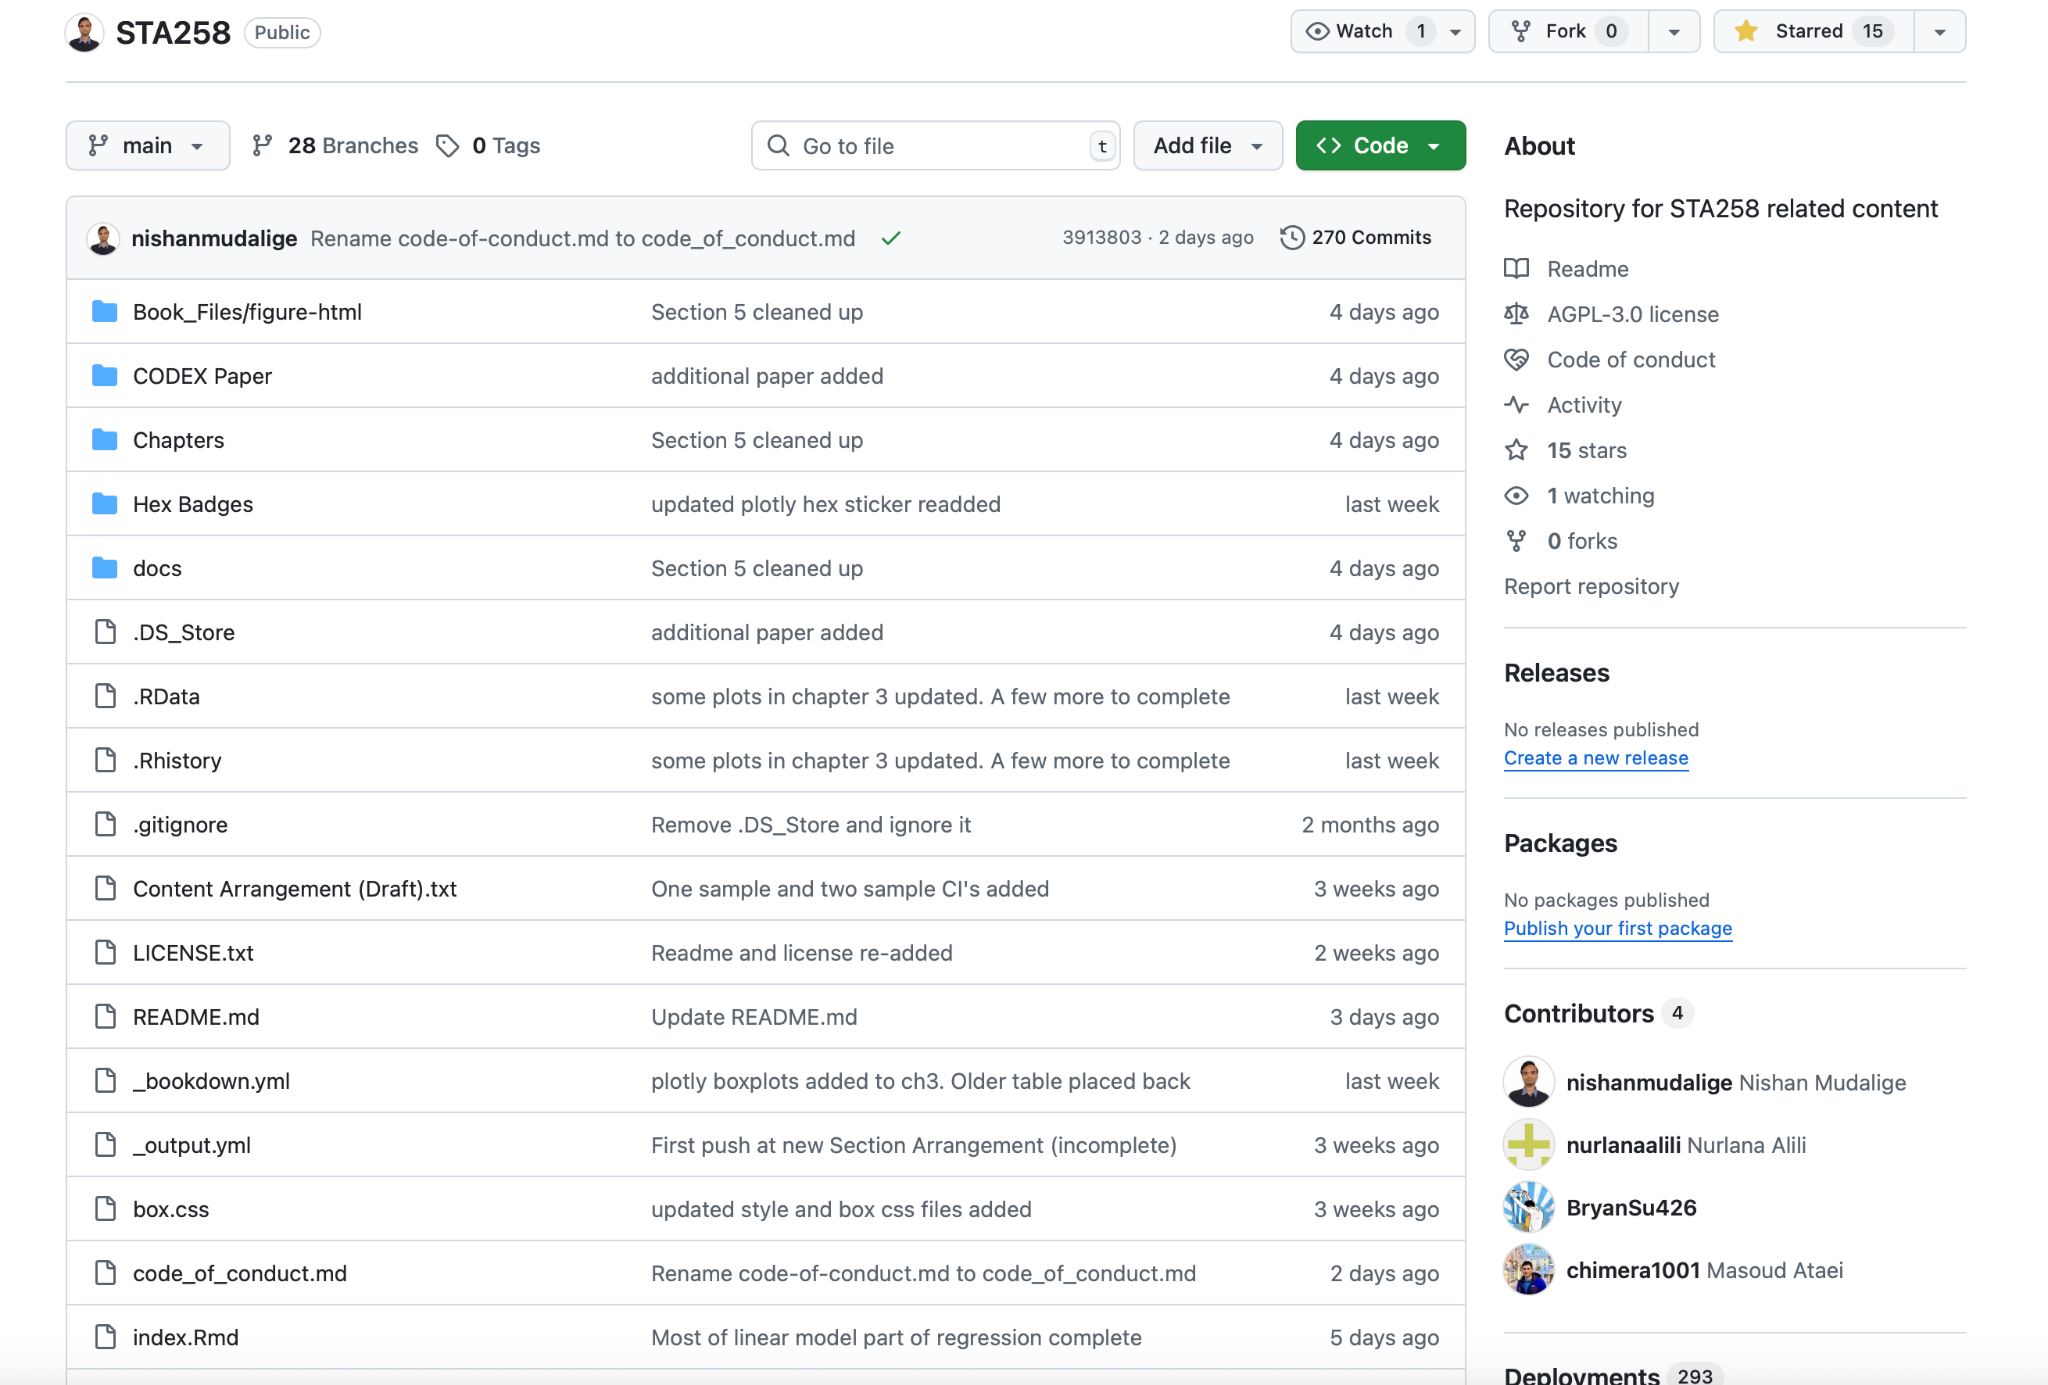
\includegraphics[width=0.7\textwidth]{Images/github-ss.png}
\end{pepadunfigure}

\section{CONTENT AND INTERACTIVE DESIGN}

The development of the e-textbook required significant planning and coordination to ensure that the final product was cohesive and pedagogically meaningful. The initial draft was largely a collection of numbered lecture notes and presentation slides. To build something more unified, we first created a full version in LaTeX, which allowed for better organization of formatting and structure. However, after reviewing the draft, we realized that the large number of chapters caused fragmentation of related content, making it more difficult for students to follow.

Through collaboration and discussion, we combined overlapping sections and reordered material into a more logical flow. This process helped reduce redundancy and resulted in a smoother experience for both students and instructors.

The final outline begins with foundational statistical concepts, including key terminology, data types, and the basic ideas behind inferential statistics. Recognizing the importance of technical skills, we included an early chapter on R programming and its practical uses. This section explains how to install R, use essential functions, and work with basic data structures and visualizations. Together, these elements provide a strong technical foundation. From there, the book progresses through core statistical methods, covering confidence intervals, hypothesis testing, and statistical power, before moving into topics such as analysis of variance, linear regression, and categorical data analysis. The structure was designed to support progressive skill-building for students while offering instructors a clear and teachable sequence of topics.

One of the most challenging aspects of the project was presenting statistical ideas visually in a way that was both accurate and engaging. At first, we used TikZ in LaTeX to create static diagrams, which worked well for simple illustrations. However, more complex concepts, such as how changes in correlation affect the shape of data, were difficult to represent using only static figures. While we could explain the theory behind these concepts, the lack of interactivity limited students’ ability to explore them meaningfully.

After encountering this limitation, we revisited our approach to visualization. We shifted to using R Markdown and Shiny to build interactive web applications. These tools allowed students to manipulate variables and observe how distributions changed in real time. Although they took time to build and required trial and error, they significantly improved the exploratory aspect of the learning experience.

To illustrate these interactive elements in practice, we developed a short lesson on histogram interpretation, skewness, and dynamic bin width adjustment. This section begins by comparing left-skewed, right-skewed, and symmetric distributions using interactive histograms, helping students build intuition about shape and spread. The lesson concludes with an app that allows students to adjust bin widths and explore how histogram appearance changes with sampling resolution (Figures 2–5).

\begin{figure}[H]
  \centering
  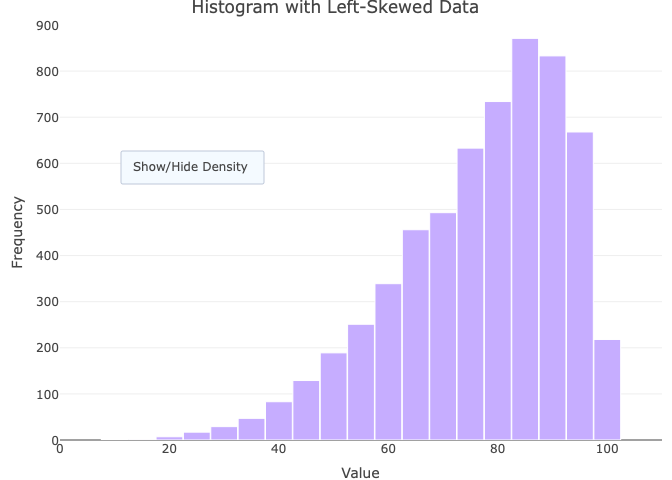
\includegraphics[width=0.75\textwidth]{Images/left.png}
  \caption{An interactive histogram displaying a left-skewed distribution. Students can toggle the kernel density overlay and observe how left-skewness shifts the bulk of the distribution toward higher values, providing a visual interpretation of negative skew.}
\end{figure}

\begin{figure}[H]
  \centering
  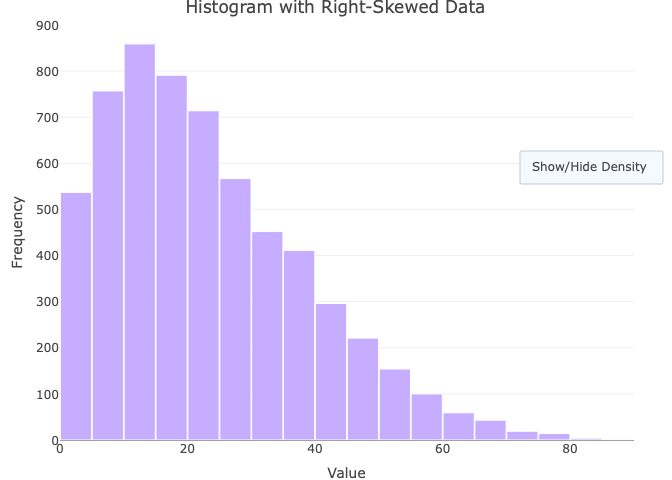
\includegraphics[width=0.75\textwidth]{Images/right.png}
  \caption{A histogram showing a right-skewed distribution. This figure enables students to identify how the majority of values cluster on the left side, with a long tail extending rightward, reinforcing the concept of positive skew.}
\end{figure}

\begin{figure}[H]
  \centering
  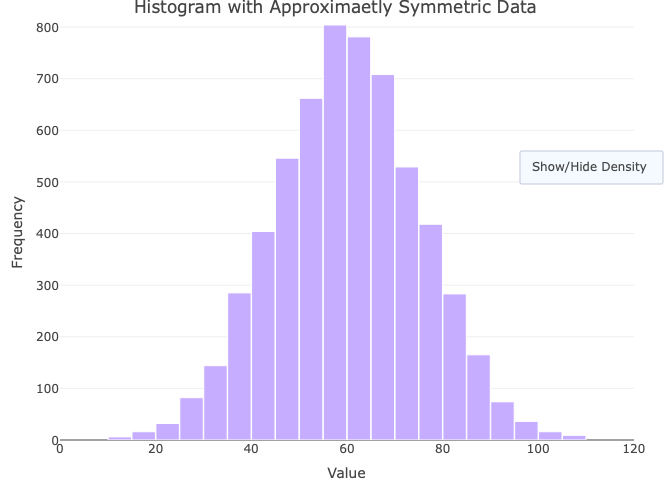
\includegraphics[width=0.75\textwidth]{Images/symm.png}
  \caption{A symmetric histogram used to contrast with skewed examples. It illustrates an approximately normal distribution with balanced tails, aiding in comparisons of central tendency and dispersion.}
\end{figure}

\begin{figure}[H]
  \centering
  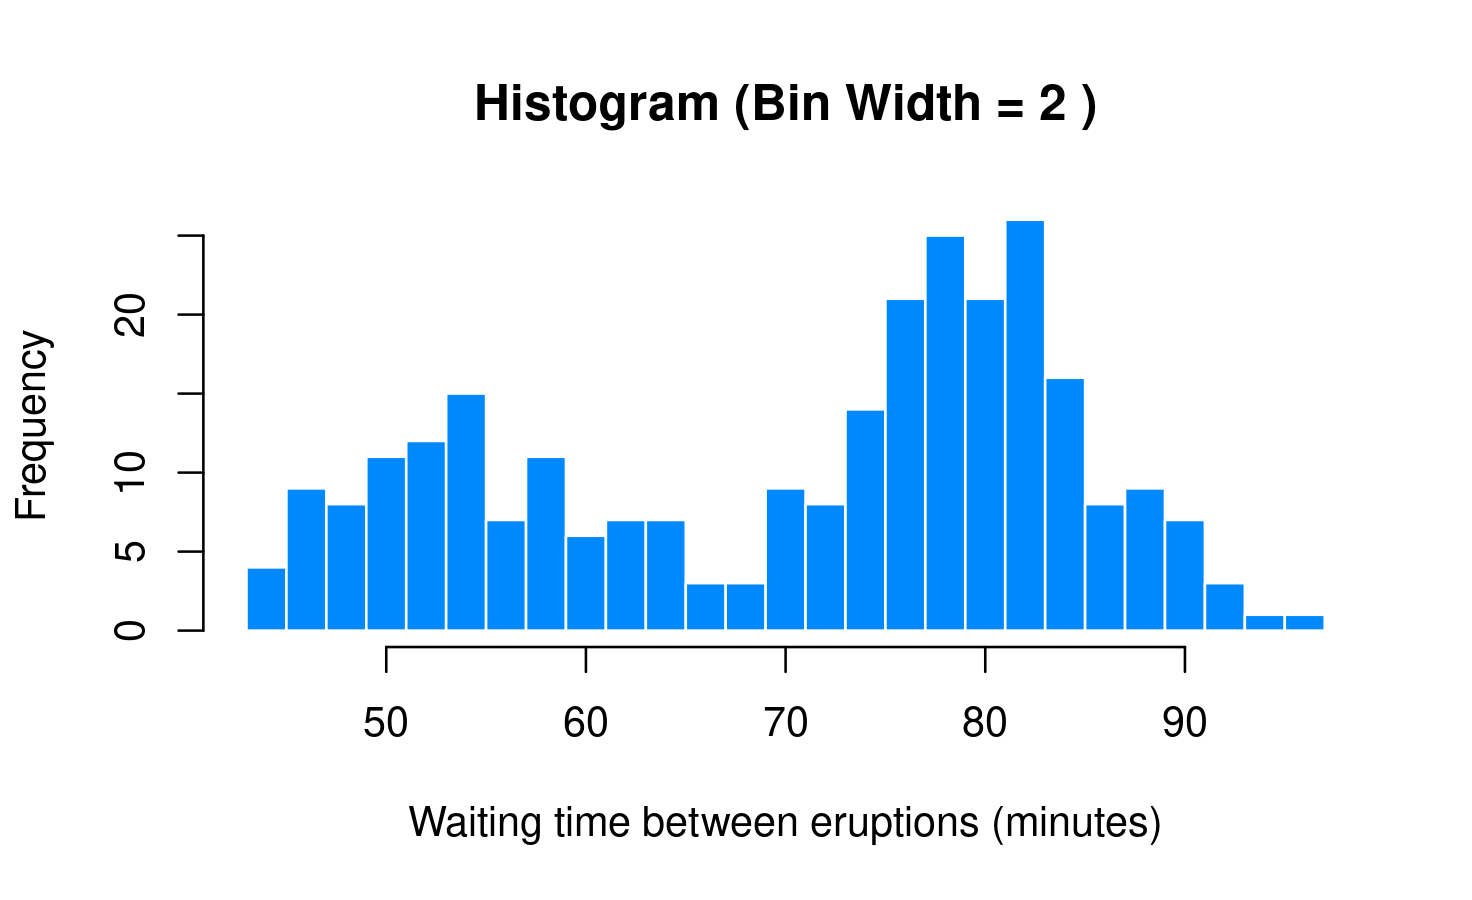
\includegraphics[width=0.75\textwidth]{Images/bin.png}
  \caption{Interactive application that allows students to adjust the bin width for a histogram built on real-world data (geyser eruption waiting times). The tool demonstrates how histogram appearance is sensitive to graphical parameters, enhancing students’ understanding of distribution shape and granularity.}
\end{figure}


One of the most rewarding parts of the project was designing the figures. Many were created using ggplot2 and are now central features of the e-book. They are visually clear, carefully styled, and interactive where appropriate. These visualizations reflect intentional design choices and help communicate complex ideas in a way that is both intuitive and accessible. Although this process was time-consuming, it was also one of the most enjoyable and educational parts of the project.

\begin{figure}[H]
  \centering
  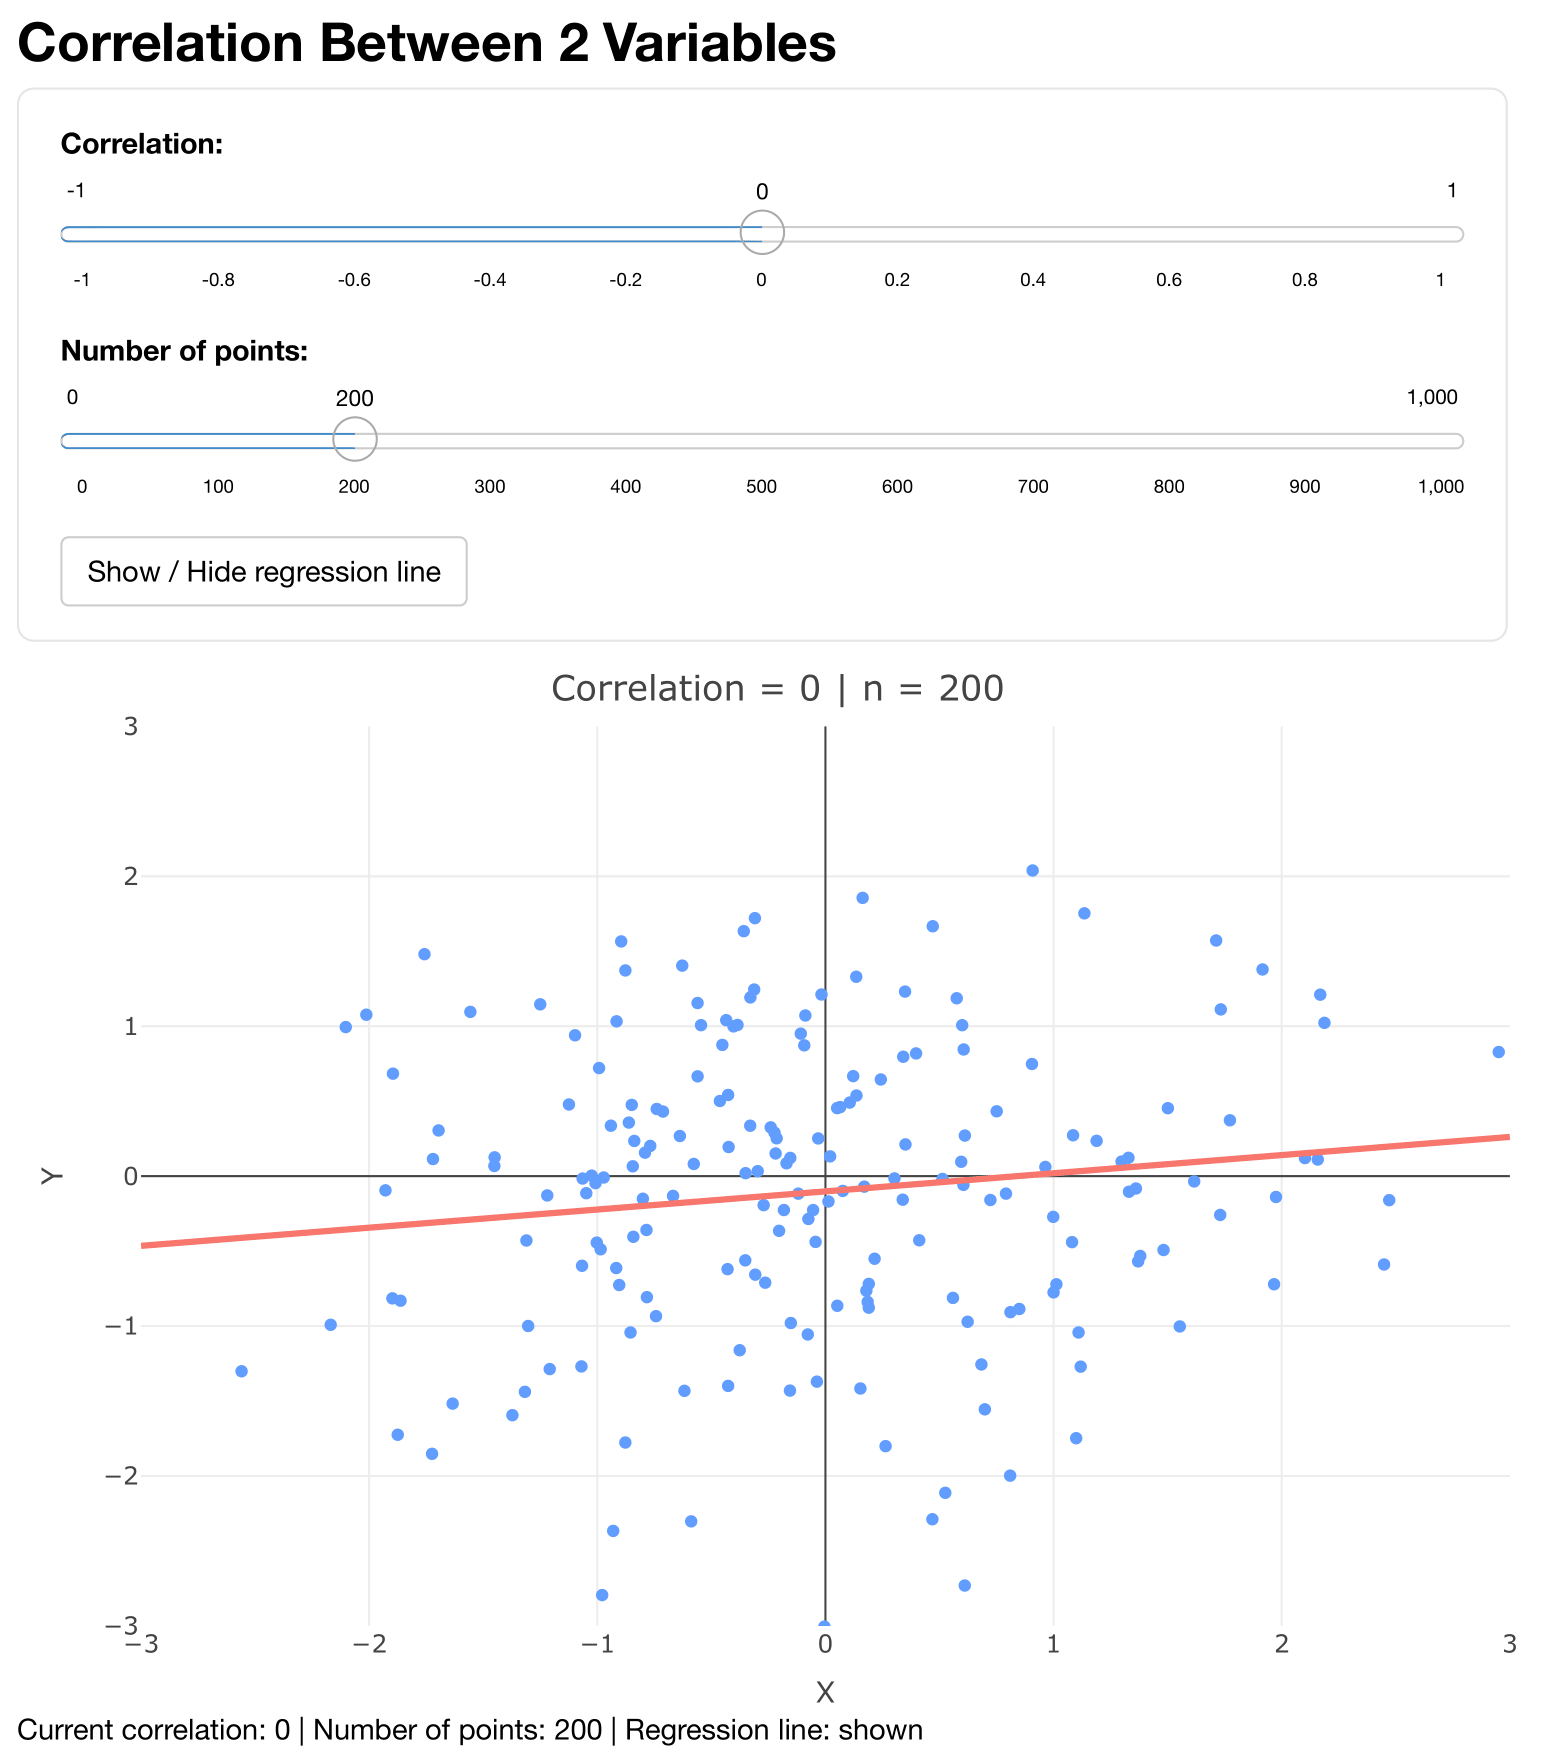
\includegraphics[width=0.7\textwidth]{Images/ch9-image.png}
  \caption{Interactive Shiny app exploring the relationship between two variables at varying correlation levels. Users can dynamically adjust the correlation coefficient and sample size, and optionally display the regression line. This tool helps students visualize how correlation strength influences the spread and direction of data points, reinforcing conceptual understanding through real-time feedback.}
\end{figure}


\section{CONCLUSION}

Beyond its technical and instructional outcomes, this project demonstrates the pedagogical potential of student-led authorship and design. By actively participating in the creation of educational content, students shift from consumers to contributors of knowledge, engaging more deeply with the subject matter.

The process required not only statistical expertise and programming fluency, but also adaptability, design thinking, and critical reflection—skills applicable in both academic and professional contexts. Through collaborative authorship, the final product embodies negotiated decisions, iterative problem-solving, and responsiveness to peer and faculty feedback.

More broadly, the project presents a replicable model of participatory curriculum development that integrates open-source tools, student initiative, and faculty mentorship to generate accessible, engaging, and adaptive learning resources.

\section{FUTURE WORK}

While the current version of the e-book successfully integrates core statistical ideas with interactive elements, there are several directions for future development. One important area is expanding the content to include more advanced topics, such as generalized linear models, non-parametric tests, or multivariate analysis. Including these topics would make the resource more useful for students in upper-year or specialized courses.

Improving accessibility and the overall user experience is another key goal. Possible next steps include optimizing the interface for mobile devices, adding text-to-speech functionality, and offering multilingual options. These features would help the e-book reach a wider range of learners from diverse backgrounds.

From a technical perspective, future versions could explore more extensive use of Shiny dashboards, where students would be able to interact with full datasets and generate real-time statistical outputs within the textbook. Additional features, such as embedded quizzes, automatic feedback on code, and user-submitted notes, could further enhance student engagement and retention of concepts.

In the long term, we hope to maintain and grow the project through continued collaboration between students and faculty. Building a clear versioning system, contributor documentation, and a guide for future authors would help ensure that the e-book remains a living resource that evolves with each new cohort.


\begin{acknowledgments}
We would like to sincerely thank Professor Nishan Mudalige, who served as the principal supervisor for this project from the very beginning. His guidance, encouragement, and consistent support played a central role in shaping both the direction and success of the e-book.

We are also grateful to Professor Masoud Ataei, whose input during the later stages of development helped refine both the technical and pedagogical aspects of the project. His feedback was thoughtful and valuable throughout.

We thank our fellow collaborators for their contributions and support, as well as the Department of Mathematical and Computational Sciences at the University of Toronto Mississauga for fostering an environment where student–faculty collaboration is encouraged and actively supported and facilitated.

Finally, we acknowledge the open-source community. The tools, documentation, and shared knowledge developed and maintained by contributors around the world made the technical side of this project achievable and rewarding.
\end{acknowledgments}

%────────────────────────────────────────────────
%— Updated bibliography command
%\printbibliography[title={REFERENCES},heading=bibintoc]

\end{document}
